%!TEX root = ../RPA_for_Creating_Program_Note.tex



\index{ふりわけ@振分け}振分けの長さ(\index{ふりわけちょう@振分長}\textbf{振分長})は、トップ側とボトム側では一般に異なる。
しかし、加工をする際には\index{ジグのちゅうしん@ジグの中心}ジグの中心に対して両者の長さの差が小さいほうが一般的には好都合である。
そうした場合の対処法として、ここでは以下のような2つの方法を考える。
\begin{enumerate}
\item
適当な厚さの\index{スペーサ}\textbf{スペーサ}を\index{ワークとジグのせってん@ワークとジグの接点}ワークとジグの接点に取り付けることで、双方の振分長を調節
\item
適当な角度に\index{テーブル}テーブルを回転することで、双方の振分長を調節
\end{enumerate}
このとき、\index{ワーク}ワークがどのように移動するかを考える。

基本的な考え方として、\index{ちゅうしんわんきょく@中心湾曲}\textbf{中心湾曲}半径$R_\mathrm c$の円の中心を原点として$\Omega$だけ回転し、次にワークとの(スペーサを装着していない側の)接点を中心に$-\theta$だけ回転したと考えることができる。
なお、ここでは話の簡単化のため、もとの振分けではトップ側よりボトム側の振分長のほうが長いものとする。




%%%%%%%%%%%%%%%%%%%%%%%%%%%%%%%%%%%%%%%%%%%%%%%%%%%%%%%%%%
%% section 1.1 %%%%%%%%%%%%%%%%%%%%%%%%%%%%%%%%%%%%%%%%%%%
%%%%%%%%%%%%%%%%%%%%%%%%%%%%%%%%%%%%%%%%%%%%%%%%%%%%%%%%%%
\modHeadsection{ジグの接点部が点の場合}
まずは簡単のため、\index{ジグ}ジグの\index{ワーク}ワークとの接点部(\pageautoref{fig:mouldOnComplexPlane1}のU$_\mathrm T$, U$_\mathrm B$の部分)は点であるとして考える。
%%%%%%%%%%%%%%%%%%%%%%%%%%%%%%%%%%%%%%%%%%%%%%%%%%%%%%%%%%
%% figure %%%%%%%%%%%%%%%%%%%%%%%%%%%%%%%%%%%%%%%%%%%%%%%%
%%%%%%%%%%%%%%%%%%%%%%%%%%%%%%%%%%%%%%%%%%%%%%%%%%%%%%%%%%
\begin{figure}[p]
\centering%
\begin{Figlandscape}
\captionsetup{width=.75\textheight}
\begin{adjustbox}{%
  addcode={\begin{minipage}{\textheight}\centering}{%
    \captionof{figure}[湾曲中心Oを原点とした複素平面上のモールド]{%
      \index{わんきょくちゅうしん@湾曲中心}湾曲中心Oを\index{げんてんO@原点O}原点とした\index{ふくそへいめん@複素平面}複素平面上のモールド\newline
      T$_\mathrm o$, T$_\mathrm i$, B$_\mathrm o$, B$_\mathrm i$, U$_\mathrm T$, U$_\mathrm B$は点、%
      $R_\mathrm c$, $R_\mathrm o$, $R_\mathrm i$, $f_\mathrm T$, $f_\mathrm B$, $l$は長さ、%
      $\alpha_{\mathrm T_\mathrm o}$, $\alpha_{\mathrm T_\mathrm i}$, $\alpha_{\mathrm U_\mathrm B}$は角度を示す。%
      \label{fig:mouldOnComplexPlane1}%
    }%
    \end{minipage}%
  },
  rotate=90,
  max width=\textwidth,
  max height=\textheight,
  keepaspectratio}
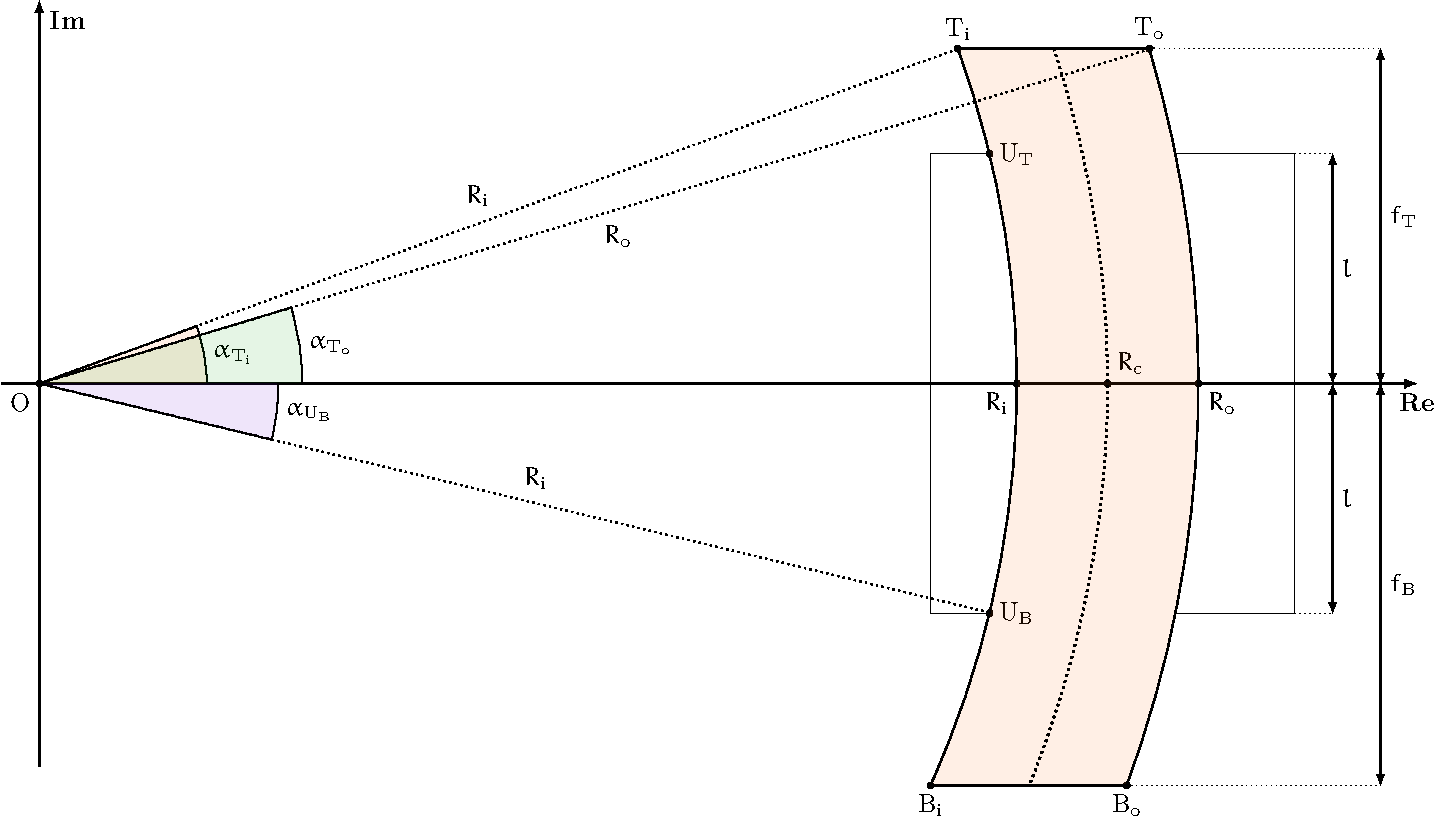
\includegraphics{./RfCPN_a1_pictures/RfCPN_p5_pictures/mouldoverall.pdf}
\end{adjustbox}
\end{Figlandscape}%
\end{figure}
%%%%%%%%%%%%%%%%%%%%%%%%%%%%%%%%%%%%%%%%%%%%%%%%%%%%%%%%%%
%%%%%%%%%%%%%%%%%%%%%%%%%%%%%%%%%%%%%%%%%%%%%%%%%%%%%%%%%%
%%%%%%%%%%%%%%%%%%%%%%%%%%%%%%%%%%%%%%%%%%%%%%%%%%%%%%%%%%



%%%%%%%%%%%%%%%%%%%%%%%%%%%%%%%%%%%%%%%%%%%%%%%%%%%%%%%%%%
%% subsection 1.1.1 %%%%%%%%%%%%%%%%%%%%%%%%%%%%%%%%%%%%%%
%%%%%%%%%%%%%%%%%%%%%%%%%%%%%%%%%%%%%%%%%%%%%%%%%%%%%%%%%%
\subsection{スペーサを用いた再振分け}
\index{モールド}モールドの湾曲における円の中心\index{O(わんきょくちゅうしん)@O(湾曲中心)}Oを\index{げんてんO@原点O}原点とした\index{ふくそへいめん@複素平面}複素平面を考える
%% footnote %%%%%%%%%%%%%%%%%%%%%
\footnote{ここでは$0 < R_\mathrm c < \infty$ ($0 < \nicefrac1{R_\mathrm c} < \infty$)としている。
$R_\mathrm c \to \infty$ ($\nicefrac1{R_\mathrm c} \to 0$)の場合、すなわち\index{わんきょくのないモールド@湾曲のないモールド}湾曲のないまっすぐなモールドの場合は、別途考える必要がある。}。
%%%%%%%%%%%%%%%%%%%%%%%%%%%%%%%%%
このとき、\pageautoref{fig:mouldOnComplexPlane1}のように、$R_\mathrm c$, $R_\mathrm i$, $R_\mathrm o$, $f_\mathrm T$, $f_\mathrm B$, $l$, $\alpha_{\mathrm T_\mathrm i}$, $\alpha_{\mathrm T_\mathrm o}$, $\alpha_{\mathrm U_\mathrm B}$をとると、
\begin{subequations}
%% label{eq:constraintUpoint1}
%% label{eq:constraintUpoint2}
\begin{gather}
  \label{eq:constraintUpoint1}
  R_\mathrm o - R_\mathrm c = R_\mathrm c - R_\mathrm i = \frac{W_x}2~, \qquad
  \IP\left(R_\mathrm oe^{i\alpha_{\mathrm T_\mathrm o}} - R_\mathrm ie^{i\alpha_{\mathrm T_\mathrm i}}\right)
  = 0~,\\
  \label{eq:constraintUpoint2}
  \sin\alpha_{\mathrm T_\mathrm i} = \frac{f_\mathrm T}{R_\mathrm i}, \qquad
  \sin\alpha_{\mathrm U_\mathrm B} = \frac l{R_\mathrm i}, \qquad
  \tan\theta = \frac{\delta_\mathrm s}{2l}~.
\end{gather}
\end{subequations}
ここで$W_x$はモールドの(AC)外径、$\delta_\mathrm s$は\index{スペーサあつ@スペーサ厚}スペーサの厚さ(\textbf{スペーサ厚})である。
このときモールドを原点Oを中心に$\Omega$だけ回転し、さらに点U$_\mathrm B$($R_\mathrm i$, $-\alpha_{\mathrm U_\mathrm B}$)を中心に$-\theta$だけ回転すると、点T$_\mathrm i$($R_\mathrm i$, $\alpha_{\mathrm T_\mathrm i}$)は、
%% label{eq:afterftUpoint}
\begin{align}
  \notag
  & e^{-i\theta}\left\{R_\mathrm ie^{i(\alpha_{\mathrm T_\mathrm i} + \Omega)} - R_\mathrm ie^{-i\alpha_{\mathrm U_\mathrm B}}\right\}
    +R_\mathrm ie^{-i\alpha_{\mathrm U_\mathrm B}}\\
  &= R_\mathrm i
     \left\{
       e^{i(\alpha_{\mathrm T_\mathrm i} + \Omega - \theta)} - e^{-i(\alpha_{\mathrm U_\mathrm B} + \theta)} + e^{-i\alpha_{\mathrm U_\mathrm B}}
     \right\}
  \label{eq:afterftUpoint}
\end{align}
に移動する。
また同様に点T$_\mathrm o$($R_\mathrm o$, $\alpha_{\mathrm T_\mathrm o}$)は
\begin{align*}
  \notag
  R_\mathrm oe^{i(\alpha_{\mathrm T_\mathrm o} + \Omega - \theta)}
  -R_\mathrm i\left\{e^{-i(\alpha_{\mathrm U_\mathrm B} + \theta)}-e^{-i\alpha_{\mathrm U_\mathrm B}}\right\}
\end{align*}
に移動する。
したがって、これらの差
\begin{align*}
  \notag
  e^{i(\Omega - \theta)}\left(R_\mathrm oe^{i\alpha_{\mathrm T_\mathrm o}} - R_\mathrm ie^{i\alpha_{\mathrm T_\mathrm i}}\right)
\end{align*}
の虚部が$0$であればよい。
つまり、\pageeqref{eq:constraintUpoint1}より、$\Omega = \theta$である
%% footnote %%%%%%%%%%%%%%%%%%%%%
\footnote{ここでは$0 \leqq \Omega, \theta < \nicefrac \pi2$としている。}。
%%%%%%%%%%%%%%%%%%%%%%%%%%%%%%%%%

スペーサを入れた後の(トップ側の)振分長は、\pageeqref{eq:afterftUpoint}の虚部を見ればよい。
\begin{align*}
  R_\mathrm i\left\{\sin\alpha_{\mathrm T_\mathrm i} + \sin(\alpha_{\mathrm U_\mathrm B} + \theta) - \sin\alpha_{\mathrm U_\mathrm B}\right\}
  &= f_\mathrm T -l
     +R_\mathrm i\left(\sin\alpha_{\mathrm U_\mathrm B}\cos\theta + \cos\alpha_{\mathrm U_\mathrm B}\sin\theta\right)\\
  &= f_\mathrm T -l+l\cdot\frac{2l}{\sqrt{4l^2+\delta_\mathrm s^2}}
     +\sqrt{R_\mathrm i^2-l^2}\cdot\frac{\delta_\mathrm s}{\sqrt{4l^2+\delta_\mathrm s^2}}\\
  &= f_\mathrm T -l+\frac{2l^2+\delta_\mathrm s\sqrt{R_\mathrm i^2-l^2}}{\sqrt{4l^2+\delta_\mathrm s^2}}~.
\end{align*}
まとめると、厚さ$\delta_\mathrm s$の\index{スペーサ}スペーサを入れた後のトップ側の\index{ふりわけちょう@振分長}振分長$f'_\mathrm T$は、
\begin{align*}
  f'_\mathrm T
  = f_\mathrm T -l
    +\frac{2l^2+\delta_\mathrm s\sqrt{\left(R_\mathrm c-\nicefrac{W_x}2\right)^2-l^2}}{\sqrt{4l^2+\delta_\mathrm s^2}}~.
\end{align*}



%%%%%%%%%%%%%%%%%%%%%%%%%%%%%%%%%%%%%%%%%%%%%%%%%%%%%%%%%%
%% subsection 1.1.2 %%%%%%%%%%%%%%%%%%%%%%%%%%%%%%%%%%%%%%
%%%%%%%%%%%%%%%%%%%%%%%%%%%%%%%%%%%%%%%%%%%%%%%%%%%%%%%%%%
\subsection{振分長が均等になるスペーサ厚}
%%%%%%%%%%%%%%%%%%%%%%%%%%%%%%%
トップ側とボトム側の\index{きんとうふりわけ@均等振分}振分長が同じになるとき、$\delta_\mathrm s$は
\begin{align*}
  f'_\mathrm T - f_\mathrm T = \frac{f_\mathrm B - f_\mathrm T}2
\end{align*}
を満たす。
これより、
\begin{align*}
  \frac{2l^2+\delta_\mathrm s\sqrt{R_\mathrm i^2-l^2}}{\sqrt{4l^2+\delta_\mathrm s^2}} = l'\qquad
  \left(l' \equiv l + \frac{f_\mathrm B-f_\mathrm T}2\right)
\end{align*}
両辺を2乗すると、
\begin{gather*}
  4l^4+\delta_\mathrm s^2\left(R_\mathrm i^2-l^2\right)+4l^2\delta_\mathrm s\sqrt{R_\mathrm i^2-l^2}
  = l'^2\left(4l^2+\delta_\mathrm s^2\right)\\
  \longrightarrow\quad
  \delta_\mathrm s^2\left(R_\mathrm i^2-l^2-l'^2\right)
  +4l^2\delta_\mathrm s\sqrt{R_\mathrm i^2-l^2} -4l^2\left(l'^2 - l^2\right)
  = 0.
\end{gather*}
$\delta_\mathrm s > 0$より、
\begin{align*}
  \delta_\mathrm s
  &= \frac{\sqrt{4l^4\left(R_\mathrm i^2-l^2\right)
                 +4l^2\left(R_\mathrm i^2-l^2-l'^2\right)\left(l'^2 - l^2\right)}
           -2l^2\sqrt{R_\mathrm i^2-l^2}}{R_\mathrm i^2-l^2-l'^2}\\
  &= 2l\cdot\frac{l'\sqrt{R_\mathrm i^2-l'^2}-l\sqrt{R_\mathrm i^2-l^2}}{R_\mathrm i^2-l^2-l'^2}
\end{align*}
まとめると、求める\index{スペーサあつ@スペーサ厚}スペーサ厚$\delta_\mathrm s$は、
\begin{align*}
  \delta_\mathrm s
  = 2l\cdot
    \frac{\displaystyle
          \left(l+\frac{f_\mathrm B-f_\mathrm T}2\right)
          \sqrt{\left(R_\mathrm c-\frac{W_x}2\right)^2
                -\left(l+\frac{f_\mathrm B-f_\mathrm T}2\right)^2}
          -l\sqrt{\left(R_\mathrm c-\frac{W_x}2\right)^2-l^2}}
         {\displaystyle
          \left(R_\mathrm c-\frac{W_x}2\right)^2-l^2
          -\left(l+\frac{f_\mathrm B-f_\mathrm T}2\right)^2}~.
\end{align*}



\clearpage
%%%%%%%%%%%%%%%%%%%%%%%%%%%%%%%%%%%%%%%%%%%%%%%%%%%%%%%%%%
%% section 20.2 %%%%%%%%%%%%%%%%%%%%%%%%%%%%%%%%%%%%%%%%%%
%%%%%%%%%%%%%%%%%%%%%%%%%%%%%%%%%%%%%%%%%%%%%%%%%%%%%%%%%%
\modHeadsection{受板がある場合}
\index{ジグ}ジグの\index{ワーク}ワークと接する部品(\index{うけいた@受板}\textbf{受板})の大きさを考慮した場合を考える。
ワークに接する側の面は半径$\rho$の円弧(\index{うけいたのけい@受板の径}受板の径), 虚軸方向の厚み(\index{うけいたのはば@受板の幅}受板の幅)は$\sigma$とする。
また受板の虚軸負方向側の面は、ジグのそれと同じ平面上にあるものとする。
%%%%%%%%%%%%%%%%%%%%%%%%%%%%%%%%%%%%%%%%%%%%%%%%%%%%%%%%%%
%% figure %%%%%%%%%%%%%%%%%%%%%%%%%%%%%%%%%%%%%%%%%%%%%%%%
%%%%%%%%%%%%%%%%%%%%%%%%%%%%%%%%%%%%%%%%%%%%%%%%%%%%%%%%%%
\begin{figure}[p]%
\begin{Figbox}[valign=top]%
\resizebox{\linewidth-35pt}{!}{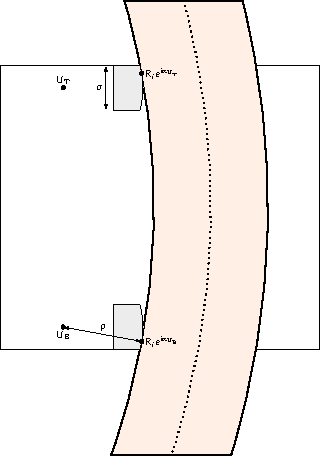
\includegraphics{./RfCPN_a1_pictures/RfCPN_p5_pictures/mouldUkeita.pdf}}%
\vfill~
\captionof{figure}[受板がある場合]{%
 \index{うけいた@受板}受板がある場合\newline
 $\rho$, $\sigma$は\index{うけいたのけい@受板の径}受板の径および\index{うけいたのはば@受板の幅}受板の幅を示し、U$_\mathrm T$, U$_\mathrm B$はそれぞれの受板の円弧の中心点を示す。
 受板があると\index{ワーク}ワークとの\index{せってん(ワークとうけいた)@接点(ワークと受板)}接点U$_\mathrm B$の位置も変化する。
 なお受板は、トップ側とボトム側で同じものであり、その片面はジグの片面と揃える形で装着されるものとする。
 \label{fig:mouldwithukeita}}
\end{Figbox}%
\end{figure}%
%%%%%%%%%%%%%%%%%%%%%%%%%%%%%%%%%%%%%%%%%%%%%%%%%%%%%%%%%%
%%%%%%%%%%%%%%%%%%%%%%%%%%%%%%%%%%%%%%%%%%%%%%%%%%%%%%%%%%
%%%%%%%%%%%%%%%%%%%%%%%%%%%%%%%%%%%%%%%%%%%%%%%%%%%%%%%%%%
\index{うけいたのちゅうしん@受板の中心}受板の径の中心を改めてU$_\mathrm B$とし、また\index{げんてんO@原点O}原点Oに対する\index{へんかく(うけいた)@偏角(受板)}偏角を改めて$-\alpha_{\mathrm U_\mathrm B}$とすると、これはU$_\mathrm B$($R_\mathrm i-\rho$, $-\alpha_{\mathrm U_\mathrm B}$)と表すことができる。
ただし、\pageeqref{eq:constraintUpoint2}は以下のようになる。
\begin{align*}
  \sin\alpha_{\mathrm U_\mathrm B} = \frac{\bar l}{R_\mathrm i-\rho}\quad, \quad
  \tan\psi = \frac{\delta_\mathrm s}{2\bar l} \quad
  \left(~\bar l \equiv l-\frac\sigma2~\right).
\end{align*}
これを原点Oを中心に$\Omega$だけ回転し、さらに点U$_\mathrm B$($R_\mathrm i-\rho$, $-\alpha_{\mathrm U_\mathrm B}$)を中心に点T$_\mathrm i$($R_\mathrm i$, $\alpha_{\mathrm T_\mathrm i}$)を$-\theta$だけ回転すると、
%% label{eq:afterftUfinite}
\begin{align}
  \notag
  & e^{-i\theta}\!
    \left\{R_\mathrm ie^{i(\alpha_{\mathrm T_\mathrm i}+\Omega)}
           -R_\mathrm i'e^{-i\alpha_{\mathrm U_\mathrm B}}\right\}
    +R_\mathrm i'e^{-i\alpha_{\mathrm U_\mathrm B}}\\
  & = R_\mathrm ie^{i(\alpha_{\mathrm T_\mathrm i}+\Omega-\theta)}
      -R_\mathrm i'\!
       \left\{e^{-i(\alpha_{\mathrm U_\mathrm B}+\theta)}-e^{-i\alpha_{\mathrm U_\mathrm B}}\right\}\qquad
    \big(R_\mathrm i' \equiv R_\mathrm i-\rho\big)
    \label{eq:afterftUfinite}
\end{align}
に移動する。
同様に点T$_\mathrm o$($R_\mathrm o$, $\alpha_{\mathrm T_\mathrm o}$)は
\begin{align*}
  R_\mathrm oe^{i(\alpha_{\mathrm T_\mathrm o}+\Omega-\theta)}
  -R_\mathrm i'\!
   \left\{e^{-i(\alpha_{\mathrm U_\mathrm B} + \theta)} - e^{-i\alpha_{\mathrm U_\mathrm B}}\right\}
\end{align*}
に移動する。
したがって、これらの差
\begin{align*}
  e^{i(\Omega-\theta)}
  \left(R_\mathrm oe^{i\alpha_{\mathrm T_\mathrm o}} - R_\mathrm ie^{i\alpha_{\mathrm T_\mathrm i}}\right)
\end{align*}
の虚部が$0$であればよい。
つまり、\pageeqref{eq:constraintUpoint1}より、受板がある場合も$\Omega = \theta$である。


%%%%%%%%%%%%%%%%%%%%%%%%%%%%%%%%%%%%%%%%%%%%%%%%%%%%%%%%%%
%% subsection 20.2.1 %%%%%%%%%%%%%%%%%%%%%%%%%%%%%%%%%%%%%
%%%%%%%%%%%%%%%%%%%%%%%%%%%%%%%%%%%%%%%%%%%%%%%%%%%%%%%%%%
\subsection{受板の接点}
\index{うけいた@受板}受板とワークとの(トップ側の)接点は、$R_\mathrm ie^{i\alpha_{\mathrm U_\mathrm B}}$で与えられる。
このとき厚さ$\delta_\mathrm s$のスペーサを取付けると、U$_\mathrm B$を中心に回転するが、それに伴い受板における接点の位置も変化する。


%%%%%%%%%%%%%%%%%%%%%%%%%%%%%%%%%%%%%%%%%%%%%%%%%%%%%%%%%%
%% subsubsection 20.2.1.1 %%%%%%%%%%%%%%%%%%%%%%%%%%%%%%%%
%%%%%%%%%%%%%%%%%%%%%%%%%%%%%%%%%%%%%%%%%%%%%%%%%%%%%%%%%%
\subsubsection{回転後のモールドの湾曲中心}
%%%%%%%%%%%%%%%%%%%%%%%%%
厚さ$\delta_\mathrm s$の\index{スペーサ}スペーサを挟むと、トップ側における\index{うけいたのちゅうしん@受板の中心}受板の円の中心U$_\mathrm B$は実軸方向に$\delta_\mathrm s$だけ移動するので、
\begin{align*}
  R_\mathrm i'e^{i\alpha_{\mathrm U_\mathrm B}}
  \quad\longrightarrow\quad
  \delta_\mathrm s+R_\mathrm i'e^{i\alpha_{\mathrm U_\mathrm B}}\ .
\end{align*}
よって、それぞれの受板の中心U$_\mathrm B$, U$_\mathrm T$を結んだ線分U$_\mathrm B$U$_\mathrm T$は、U$_\mathrm B$を中心に$-\psi$だけ傾いた線分U$_\mathrm B'$U$_\mathrm T'$となる
%% footnote %%%%%%%%%%%%%%%%%%%%%
\footnote{%
U$_\mathrm B'$U$_\mathrm T'$の長さは$\bar l\sec\psi$であり、U$_\mathrm B$U$_\mathrm T$の長さ$\bar l$より長くなることに注意。}。
%%%%%%%%%%%%%%%%%%%%%%%%%%%%%%%%%
\index{かいてんごのわんきょくちゅうしん@回転後の湾曲中心}回転後のワークの湾曲中心は、この線分の垂直二等分線上にあり、またそれぞれの受板の中心から$R_\mathrm i'$の距離の位置にある。
つまり、この傾いた線分U$_\mathrm B'$U$_\mathrm T'$の中点から、角度$\pi-\psi$, 大きさ$\sqrt{R_\mathrm i'^2-\frac{\delta_\mathrm s^2+(2\bar l)^2}4}$の位置に移動する。
したがって、回転後における湾曲中心O$'$は、
%% label{eq:afterOrgin}
\begin{align}
  \notag
  & \frac{\delta_\mathrm s}2+\sqrt{R_\mathrm i'^2-\bar l^2}
    +\sqrt{R_\mathrm i'^2-\frac{\delta_\mathrm s^2+(2\bar l)^2}4}e^{i(\pi-\psi)}\\
  & = \frac{\delta_\mathrm s}2+\sqrt{R_\mathrm i'^2-\bar l^2}-\sqrt{R_\mathrm i'^2-\frac{\delta_\mathrm s^2+(2\bar l)^2}4}\cos\psi
      +i\sqrt{R_\mathrm i'^2-\frac{\delta_\mathrm s^2+(2\bar l)^2}4}\sin\psi\ .
    \label{eq:afterOrgin}
\end{align}


\clearpage
%%%%%%%%%%%%%%%%%%%%%%%%%%%%%%%%%%%%%%%%%%%%%%%%%%%%%%%%%%
%% subsubsection 19.2.1.2 %%%%%%%%%%%%%%%%%%%%%%%%%%%%%%%%
%%%%%%%%%%%%%%%%%%%%%%%%%%%%%%%%%%%%%%%%%%%%%%%%%%%%%%%%%%
\subsubsection{回転後の接点(トップ側)}
\index{かいてんごのうけいたのちゅうしん@回転後の受板の中心}回転後のトップ側における受板の中心U$_\mathrm T'$と\index{かいてんごのわんきょくちゅうしん@回転後の湾曲中心}湾曲中心O$'$との差をとると、
\begin{align*}
  \frac{\delta_\mathrm s}2+\sqrt{R_\mathrm i'^2-\frac{\delta_\mathrm s^2+(2\bar l)^2}4}\cos\psi
  +i\left\{\bar l-\sqrt{R_\mathrm i'^2-\frac{\delta_\mathrm s^2+(2\bar l)^2}4}\sin\psi\right\}
  = R_\mathrm i'e^{i\alpha'_{\mathrm U_\mathrm T}}\ .
\end{align*}
ここで、
\begin{align*}
  \tan\alpha'_{\mathrm U_\mathrm T}
  = \frac{\displaystyle\bar l-\sqrt{R_\mathrm i'^2-\frac{\delta_\mathrm s^2+(2\bar l)^2}4}\sin\psi}
         {\displaystyle\frac{\delta_\mathrm s}2+\sqrt{R_\mathrm i'^2-\frac{\delta_\mathrm s^2+(2\bar l)^2}4}\cos\psi}\ .
\end{align*}
%%%%%%%%%%%%%%%%%%%%%%%%%%%%%%%%%%%%%%%%%%%%%%%%%%%%%%%%%%
%% hosoku %%%%%%%%%%%%%%%%%%%%%%%%%%%%%%%%%%%%%%%%%%%%%%%%
%%%%%%%%%%%%%%%%%%%%%%%%%%%%%%%%%%%%%%%%%%%%%%%%%%%%%%%%%%
\begin{hosoku}
これの大きさは、$\delta_\mathrm s\cos\psi-2\bar l\sin\psi = 0$より、
\begin{align*}
  \left\{\frac{\delta_\mathrm s}2+\sqrt{R_\mathrm i'^2-\frac{\delta_\mathrm s^2+(2\bar l)^2}4}\cos\psi\right\}^2
  +\left\{\bar l-\sqrt{R_\mathrm i'^2-\frac{\delta_\mathrm s^2+(2\bar l)^2}4}\sin\psi\right\}^2
  = R_\mathrm i'^2\ .
\end{align*}
\end{hosoku}
%%%%%%%%%%%%%%%%%%%%%%%%%%%%%%%%%%%%%%%%%%%%%%%%%%%%%%%%%%
%%%%%%%%%%%%%%%%%%%%%%%%%%%%%%%%%%%%%%%%%%%%%%%%%%%%%%%%%%
%%%%%%%%%%%%%%%%%%%%%%%%%%%%%%%%%%%%%%%%%%%%%%%%%%%%%%%%%%
よって、回転後の接点は以下で与えられる。
\begin{align*}
  &  R_\mathrm ie^{i\alpha'_{\mathrm U_\mathrm T}}
     +\frac{\delta_\mathrm s}2+\sqrt{R_\mathrm i'^2-\bar l^2}-\sqrt{R_\mathrm i'^2-\frac{\delta_\mathrm s^2+(2\bar l)^2}4}\cos\psi
     +i\sqrt{R_\mathrm i'^2-\frac{\delta_\mathrm s^2+(2\bar l)^2}4}\sin\psi\\
  &= \delta_\mathrm s+R_\mathrm i'e^{i\alpha_{\mathrm U_\mathrm B}}+\rho e^{i\alpha'_{\mathrm U_\mathrm T}}\ .
\end{align*}


%%%%%%%%%%%%%%%%%%%%%%%%%%%%%%%%%%%%%%%%%%%%%%%%%%%%%%%%%%
%% subsubsection 1.2.1.3 %%%%%%%%%%%%%%%%%%%%%%%%%%%%%%%%%
%%%%%%%%%%%%%%%%%%%%%%%%%%%%%%%%%%%%%%%%%%%%%%%%%%%%%%%%%%
\subsubsection{回転後の接点(ボトム側)}
回転後のボトム側における受板の中心U$_\mathrm B$と\index{わんきょくちゅうしん@湾曲中心}湾曲中心O$'$との差をとると、
\begin{align*}
  -\frac{\delta_\mathrm s}2+\sqrt{R_\mathrm i'^2-\frac{\delta_\mathrm s^2+(2\bar l)^2}4}\cos\psi
  -i\left\{\bar l+\sqrt{R_\mathrm i'^2-\frac{\delta_\mathrm s^2+(2\bar l)^2}4}\sin\psi\right\}
  = R_\mathrm i'e^{-i\alpha'_{\mathrm U_\mathrm B}}
\end{align*}
ここで、
\begin{align*}
  \tan\alpha'_{\mathrm U_\mathrm B}
  = \frac{\displaystyle\bar l+\sqrt{R_\mathrm i'^2-\frac{\delta_\mathrm s^2+(2\bar l)^2}4}\sin\psi}
         {\displaystyle-\frac{\delta_\mathrm s}2+\sqrt{R_\mathrm i'^2-\frac{\delta_\mathrm s^2+(2\bar l)^2}4}\cos\psi}
\end{align*}
よって、回転後の接点は以下で与えられる。
%% label{eq:afterUBcontact}
\begin{align}
  \notag
  &  R_\mathrm ie^{-i\alpha'_{\mathrm U_\mathrm B}}
     +\frac{\delta_\mathrm s}2+\sqrt{R_\mathrm i'^2-\bar l^2}-\sqrt{R_\mathrm i'^2-\frac{\delta_\mathrm s^2+(2\bar l)^2}4}\cos\psi
     +i\sqrt{R_\mathrm i'^2-\frac{\delta_\mathrm s^2+(2\bar l)^2}4}\sin\psi\\
  &= R_\mathrm i'e^{-i\alpha_{\mathrm U_\mathrm B}}+\rho e^{-i\alpha'_{\mathrm U_\mathrm B}}
   \label{eq:afterUBcontact}
\end{align}
%%%%%%%%%%%%%%%%%%%%%%%%%%%%%%%%%%%%%%%%%%%%%%%%%%%%%%%%%%
%% hosoku %%%%%%%%%%%%%%%%%%%%%%%%%%%%%%%%%%%%%%%%%%%%%%%%
%%%%%%%%%%%%%%%%%%%%%%%%%%%%%%%%%%%%%%%%%%%%%%%%%%%%%%%%%%
\begin{hosoku}
辺の長さが$R_i'$, $R_i'$, $2\bar l$の二等辺三角形$\triangle$OU$_\mathrm B$U$_\mathrm T$の部分が、回転後には辺の長さ$R_i'$, $R_i'$, $\sqrt{\delta_\mathrm s^2+(2\bar l)^2}$の二等辺三角形$\triangle$O$'$U$_\mathrm B'$U$_\mathrm T'$となる。
実際、$\cos2a = 1-2\sin^2\!a$より、
\begin{align*}
  \sin^2\frac{\alpha'_{\mathrm U_\mathrm T}+\alpha'_{\mathrm U_\mathrm B}}2
  = \frac{\delta_\mathrm s^2+(2\bar l)^2}{4R_\mathrm i'^2}\ .
\end{align*}
\end{hosoku}
%%%%%%%%%%%%%%%%%%%%%%%%%%%%%%%%%%%%%%%%%%%%%%%%%%%%%%%%%%
%%%%%%%%%%%%%%%%%%%%%%%%%%%%%%%%%%%%%%%%%%%%%%%%%%%%%%%%%%
%%%%%%%%%%%%%%%%%%%%%%%%%%%%%%%%%%%%%%%%%%%%%%%%%%%%%%%%%%


%%%%%%%%%%%%%%%%%%%%%%%%%%%%%%%%%%%%%%%%%%%%%%%%%%%%%%%%%%
%% subsection 1.2.2 %%%%%%%%%%%%%%%%%%%%%%%%%%%%%%%%%%%%%%
%%%%%%%%%%%%%%%%%%%%%%%%%%%%%%%%%%%%%%%%%%%%%%%%%%%%%%%%%%
\subsection{スペーサによるモールドの回転角}
厚さ$\delta_\mathrm s$の\index{スペーサ}スペーサを挿入すると、\index{わんきょくちゅうしん@湾曲中心}湾曲中心Oは、U$_\mathrm B$を中心に$-\left(\alpha'_{\mathrm U_\mathrm B}\!-\alpha_{\mathrm U_\mathrm B}\right)$だけ回転する。
実際、
\begin{align*}
  -R_\mathrm i'e^{-i\alpha'_{\mathrm U_\mathrm B}}+R_\mathrm i'e^{-i\alpha_{\mathrm U_\mathrm B}}
  &= R_\mathrm i'(\cos\alpha_{\mathrm U_\mathrm B}-\cos\alpha'_{\mathrm U_\mathrm B})
     +iR_\mathrm i'(\sin\alpha'_{\mathrm U_\mathrm B}-\sin\alpha_{\mathrm U_\mathrm B})
\end{align*}
であり、これは\index{かいてんごのわんきょくちゅうしん@回転後の湾曲中心}回転後の湾曲中心\pageeqref{eq:afterOrgin}に一致する。
つまり、$\alpha'_{\mathrm U_\mathrm B}\!-\alpha_{\mathrm U_\mathrm B}$が$\theta$に相当する。
%%%%%%%%%%%%%%%%%%%%%%%%%%%%%%%%%%%%%%%%%%%%%%%%%%%%%%%%%%
%% hosoku %%%%%%%%%%%%%%%%%%%%%%%%%%%%%%%%%%%%%%%%%%%%%%%%
%%%%%%%%%%%%%%%%%%%%%%%%%%%%%%%%%%%%%%%%%%%%%%%%%%%%%%%%%%
\begin{hosoku}
トップ側の接点U$_\mathrm T'$とボトム側の接点U$_\mathrm B'$の差をとると、
\begin{align*}
  R_\mathrm i\left(e^{i\alpha_{\mathrm U_\mathrm T}'}-e^{-i\alpha'_{\mathrm U_\mathrm B}}\right)
  &= \frac{R_\mathrm i'+\rho}{R_\mathrm i'}\left\{\delta_\mathrm s+i(2\bar l)\right\}
   = \frac{R_\mathrm i}{R_\mathrm i'}\sqrt{\delta_\mathrm s^2+(2\bar l)^2}e^{i(\nicefrac\pi2-\psi)}\ .
\end{align*}
したがって、厚さ$\delta_\mathrm s$のスペーサを挿入すると、両接点を通る直線は$-\psi$だけ傾くことがわかる。
また、その長さは受板中心間U$_\mathrm T'$U$_\mathrm B'$の距離$\sqrt{\delta_\mathrm s^2+(2\bar l)^2}$の$\nicefrac{R_i}{R_i'}$倍になっていることも確かめられる。
\end{hosoku}
%%%%%%%%%%%%%%%%%%%%%%%%%%%%%%%%%%%%%%%%%%%%%%%%%%%%%%%%%%
%%%%%%%%%%%%%%%%%%%%%%%%%%%%%%%%%%%%%%%%%%%%%%%%%%%%%%%%%%
%%%%%%%%%%%%%%%%%%%%%%%%%%%%%%%%%%%%%%%%%%%%%%%%%%%%%%%%%%


%%%%%%%%%%%%%%%%%%%%%%%%%%%%%%%%%%%%%%%%%%%%%%%%%%%%%%%%%%
%% subsection 1.2.3 %%%%%%%%%%%%%%%%%%%%%%%%%%%%%%%%%%%%%%
%%%%%%%%%%%%%%%%%%%%%%%%%%%%%%%%%%%%%%%%%%%%%%%%%%%%%%%%%%
\subsection{スペーサによる再振分け}

%%%%%%%%%%%%%%%%%%%%%%%%%%%%%%%%%%%%%%%%%%%%%%%%%%%%%%%%%%
%% subsubsection 1.2.3.1 %%%%%%%%%%%%%%%%%%%%%%%%%%%%%%%%%
%%%%%%%%%%%%%%%%%%%%%%%%%%%%%%%%%%%%%%%%%%%%%%%%%%%%%%%%%%
\subsubsection{再振分長}
\index{スペーサ}スペーサを入れた後のトップ側の\index{ふりわけちょう@振分長}振分長(\index{さいふりわけちょう@再振分長}\textbf{再振分長})$f'_\mathrm T$は、\pageeqref{eq:afterftUfinite}の虚部を見ればよい。
回転角は$-(\alpha'_{\mathrm U_\mathrm B}-\alpha_{\mathrm U_\mathrm B})$なので、
\begin{align*}
  f'_\mathrm T
  = R_\mathrm i\sin\alpha_{\mathrm T_\mathrm i}
    +R_\mathrm i'\left(\sin\alpha'_{\mathrm U_\mathrm B}-\sin\alpha_{\mathrm U_\mathrm B}\right)
  &= f_\mathrm T+\sqrt{R_\mathrm i'^2-\frac{\delta_\mathrm s^2+(2\bar l)^2}4}\sin\psi\\
  &= f_\mathrm T+\sqrt{R_\mathrm i'^2-\frac{\delta_\mathrm s^2+(2\bar l)^2}4}\frac{\delta_\mathrm s}{\sqrt{\delta_\mathrm s^2+(2\bar l)^2}}\ .
\end{align*}

%%%%%%%%%%%%%%%%%%%%%%%%%%%%%%%%%%%%%%%%%%%%%%%%%%%%%%%%%%
%% subsubsection 1.2.3.2 %%%%%%%%%%%%%%%%%%%%%%%%%%%%%%%%%
%%%%%%%%%%%%%%%%%%%%%%%%%%%%%%%%%%%%%%%%%%%%%%%%%%%%%%%%%%
\subsubsection{モールドの移動距離}
\pageeqref{eq:afterftUfinite}の実部は、
\begin{align*}
  & R_\mathrm i\cos\alpha_{\mathrm T_\mathrm i}
    -R_\mathrm i'(\cos\alpha'_{\mathrm U_\mathrm B}-\cos\alpha_{\mathrm U_\mathrm B})\\
  & = \sqrt{R_\mathrm i^2-f_\mathrm T^2}+\frac{\delta_\mathrm s}2+\sqrt{R_\mathrm i'^2-\bar l^2}
      -\sqrt{R_\mathrm i'^2-\frac{\delta_\mathrm s^2+(2\bar l)^2}4}\cos\psi
\end{align*}
となる。
よって、\index{スペーサ}スペーサを挿入することにより、ワークは水平・鉛直方向にそれぞれ、
\begin{subequations}
%% label{eq:spacerMoveHdistance}
\begin{alignat}{2}
  \label{eq:spacerMoveHdistance}
  \text{水平方向:}\quad
  & \frac{\delta_\mathrm s}2+\sqrt{R_\mathrm i'^2-\bar l^2}-\sqrt{R_\mathrm i'^2-\frac{\delta_\mathrm s^2+(2\bar l)^2}4}\frac{2\bar l}{\sqrt{\delta_\mathrm s^2+(2\bar l)^2}}\\
  \text{鉛直方向:}\quad
  & \sqrt{R_\mathrm i'^2-\frac{\delta_\mathrm s^2+(2\bar l)^2}4}\frac{\delta_\mathrm s}{\sqrt{\delta_\mathrm s^2+(2\bar l)^2}}
\end{alignat}
\end{subequations}
だけ移動することがわかる。



%\clearpage
%%%%%%%%%%%%%%%%%%%%%%%%%%%%%%%%%%%%%%%%%%%%%%%%%%%%%%%%%%
%% subsection 1.2.4 %%%%%%%%%%%%%%%%%%%%%%%%%%%%%%%%%%%%%%
%%%%%%%%%%%%%%%%%%%%%%%%%%%%%%%%%%%%%%%%%%%%%%%%%%%%%%%%%%
\subsection{再振分長が均等になるスペーサ厚}
トップ側とボトム側の\index{きんとうふりわけ@均等振分}振分長が同じになるとき、$\delta_\mathrm s$は
\begin{align*}
  \sqrt{R_\mathrm i'^2-\frac{\delta_\mathrm s^2+(2\bar l)^2}4}\frac{\delta_\mathrm s}{\sqrt{\delta_\mathrm s^2+(2\bar l)^2}} = f_d \qquad
  \left(f_d \equiv \frac{f_\mathrm B-f_\mathrm T}2\right)\ .
\end{align*}
を満たす。
両辺を2乗して$-4$倍すると、
\begin{align*}
  \delta_\mathrm s^2\left\{\delta_\mathrm s^2+(2\bar l)^2-4R_\mathrm i'^2\right\}+4f_d^2\left\{\delta_\mathrm s^2+(2\bar l)^2\right\}
  & = \delta_\mathrm s^4-2\left\{2R_\mathrm i'^2-2\bar l^2-2f_d^2\right\}\delta_\mathrm s^2+4f_d^2(2\bar l)^2\\
  & = 0\ .
\end{align*}
したがって、$f_\mathrm T = f_\mathrm B$ ($f_d = 0$)のとき$\delta_\mathrm s = 0$であることを考慮して、
\begin{align*}
  \delta_\mathrm s^2
  &= 2\left\{
       R_\mathrm i'^2-\bar l^2-f_d^2-\sqrt{\left(R_\mathrm i'^2-\bar l^2-f_d^2\right)^2-4f_d^2\bar l^2}\,
     \right\}\\
  &= \left(\sqrt{R_\mathrm i'^2-(\bar l-f_d)^2}-\sqrt{R_\mathrm i'^2-(\bar l+f_d)^2}\,\right)^2.
\end{align*}
なお、これはワークが水平・鉛直方向にそれぞれ、
\begin{align*}
  \text{水平方向:}~\frac{\delta_\mathrm s}2+\sqrt{R_\mathrm i^2-\bar l^2}-\frac{2\bar l}{\delta_\mathrm s}f_d\quad(\delta_\mathrm s>0)\ , \qquad
  \text{鉛直方向:}~\frac{f_\mathrm B-f_\mathrm T}2
\end{align*}
だけ移動することを意味する。
%%%%%%%%%%%%%%%%%%%%%%%%%%%%%%%%%%%%%%%%%%%%%%%%%%%%%%%%%%
%% hosoku %%%%%%%%%%%%%%%%%%%%%%%%%%%%%%%%%%%%%%%%%%%%%%%%
%%%%%%%%%%%%%%%%%%%%%%%%%%%%%%%%%%%%%%%%%%%%%%%%%%%%%%%%%%
\begin{hosoku}
改めてまとめると、厚さ$\delta_\mathrm s$のスペーサを(トップ側に)挿入した後の\index{トップふりわけちょう@トップ振分長}トップ側の振分長$f_\mathrm T'$は、
\begin{align*}
  f_\mathrm T'
  = f_\mathrm T+\sqrt{R_\mathrm i'^2-\frac{\delta_\mathrm s^2+(2\bar l)^2}4}\frac{\delta_\mathrm s}{\sqrt{\delta_\mathrm s^2+(2\bar l)^2}}\ .
\end{align*}
トップ側とボトム側の\index{きんとうふりわけ@均等振分}振分長が均等になるときの\index{スペーサあつ@スペーサ厚}スペーサ厚$\delta_\mathrm s'$は、
\begin{align*}
  \delta_\mathrm s' = \sqrt{R_\mathrm i'^2-(\bar l-f_d)^2}-\sqrt{R_\mathrm i'^2-(\bar l+f_d)^2}\ .
\end{align*}
ここで、
\begin{align*}
  R_\mathrm i' = R_\mathrm c-\frac{W_x}2-\rho\ ,\quad
  \bar l = l-\frac\sigma2\ ,\quad
  f_d = \frac{f_\mathrm B-f_\mathrm T}2\ .
\end{align*}
\end{hosoku}
%%%%%%%%%%%%%%%%%%%%%%%%%%%%%%%%%%%%%%%%%%%%%%%%%%%%%%%%%%
%%%%%%%%%%%%%%%%%%%%%%%%%%%%%%%%%%%%%%%%%%%%%%%%%%%%%%%%%%
%%%%%%%%%%%%%%%%%%%%%%%%%%%%%%%%%%%%%%%%%%%%%%%%%%%%%%%%%%



\clearpage
%%%%%%%%%%%%%%%%%%%%%%%%%%%%%%%%%%%%%%%%%%%%%%%%%%%%%%%%%%
%% section 21.3 %%%%%%%%%%%%%%%%%%%%%%%%%%%%%%%%%%%%%%%%%%
%%%%%%%%%%%%%%%%%%%%%%%%%%%%%%%%%%%%%%%%%%%%%%%%%%%%%%%%%%
\modHeadsection{テーブルの回転による振分長の調節}
これまでトップ・ボトム振分長の差を小さくするために\index{スペーサ}スペーサを用いる手法を考えてきた。
スペーサを取付けることは、本質的にはボトム側の\index{うけいた@受板}受板の点U$_\mathrm B$を中心に回転しているということである。
このとき回転の中心はU$_\mathrm B$である必要はなく、他の点でも問題ない。
したがって、スペーサを用いて回転をしなくても、\index{テーブル}テーブルそのものを回転するという手法が考えられる。
これは回転の中心が、受板の点U$_\mathrm B$から\index{テーブルちゅうしん@テーブル中心}\textbf{テーブル中心}Pに変わることに相当する。

\index{うけいたのちゅうしん@受板の中心}受板の中心U$_\mathrm B$と、テーブル中心Pとの実軸方向の距離を$\varDelta$とすると、テーブル中心Pの$X$座標$\varDelta'$は次で与えられる。
%% label{eq:tableCenter}
\begin{align}
  \label{eq:tableCenter}
  \varDelta'
  = \varDelta+R_\mathrm i'\cos\alpha_{\mathrm U_\mathrm B} = \varDelta+\sqrt{R_\mathrm i'^2-\bar l^2}\ .
\end{align}
\index{トップがわのCがわそとたんてん@トップ側のC側外端点}トップ側のC側外端点T$_\mathrm i$($R_\mathrm i$, $\alpha_{\mathrm T_\mathrm i}$)を、原点Oを中心に$\Omega$だけ回転し、さらに点P\,($\varDelta'$, $0$)を中心に$-\theta$だけ回転すると、
\begin{align}
  \label{eq:afterfttable}
  e^{-i\theta}\left\{R_\mathrm i^{i(\alpha_{\mathrm T_\mathrm i}+\Omega)}-\varDelta'\right\}+\varDelta'
  = R_\mathrm ie^{i(\alpha_{\mathrm T_\mathrm i}+\Omega-\theta)}+\varDelta'\left(1-e^{-i\theta}\right)
\end{align}
に移動する。
同様に、\index{トップがわのAがわそとたんてん@トップ側のA側外端点}トップ側のA側外端点T$_\mathrm o$($R_\mathrm o$, $\alpha_{\mathrm T_\mathrm o}$)は、
\begin{align*}
  e^{-i\theta}\!\left\{R_\mathrm o^{i(\alpha_{\mathrm T_\mathrm o}+\Omega)}-\varDelta'\right\}+\varDelta'
  = R_\mathrm ie^{i(\alpha_{\mathrm T_\mathrm o}+\Omega-\theta)}+\varDelta'\!\left(1-e^{-i\theta}\right)
\end{align*}
に移動する。
したがって、これらの差
\begin{align*}
  e^{i(\Omega-\theta)}
  \left(R_\mathrm oe^{i\alpha_{\mathrm T_\mathrm o}}-R_\mathrm ie^{i\alpha_{\mathrm T_\mathrm i}}\right)
\end{align*}
の虚部が$0$であればよい。
よって\pageeqref{eq:constraintUpoint1}より、この場合も$\Omega = \theta$となる。


%%%%%%%%%%%%%%%%%%%%%%%%%%%%%%%%%%%%%%%%%%%%%%%%%%%%%%%%%%
%% subsection 21.3.1 %%%%%%%%%%%%%%%%%%%%%%%%%%%%%%%%%%%%%
%%%%%%%%%%%%%%%%%%%%%%%%%%%%%%%%%%%%%%%%%%%%%%%%%%%%%%%%%%
\subsection{回転後のモールドの湾曲中心および受板との接点}

%%%%%%%%%%%%%%%%%%%%%%%%%%%%%%%%%%%%%%%%%%%%%%%%%%%%%%%%%%
%% subsubsection 21.3.1.1 %%%%%%%%%%%%%%%%%%%%%%%%%%%%%%%%
%%%%%%%%%%%%%%%%%%%%%%%%%%%%%%%%%%%%%%%%%%%%%%%%%%%%%%%%%%
\subsubsection{回転後のモールドの湾曲中心}
\index{かいてんごのわんきょくちゅうしん@回転後の湾曲中心}回転後の湾曲中心O$'$は、点Pを中心に$-\theta$だけ回転するので、
\begin{align*}
  \varDelta'\!\left(1-e^{-i\theta}\right) = \varDelta'(1-\cos\theta)+i\varDelta'\sin\theta\ .
\end{align*}

%%%%%%%%%%%%%%%%%%%%%%%%%%%%%%%%%%%%%%%%%%%%%%%%%%%%%%%%%%
%% subsubsection 21.3.1.2 %%%%%%%%%%%%%%%%%%%%%%%%%%%%%%%%
%%%%%%%%%%%%%%%%%%%%%%%%%%%%%%%%%%%%%%%%%%%%%%%%%%%%%%%%%%
\subsubsection{回転後の接点}
回転後におけるトップ側の\index{ワークとうけいたのせってん@ワークと受板の接点}受板との接点は、点Pを中心に$-\theta$だけ回転するので、
\begin{align*}
  &  e^{-i\theta}\left(R_\mathrm ie^{i\alpha_{\mathrm U_\mathrm B}}-\varDelta'\right)+\varDelta'\\
  &= R_\mathrm ie^{i(\alpha_{\mathrm U_\mathrm B}-\theta)}+\varDelta'\!\left(1-e^{-i\theta}\right)\\
  &= R_\mathrm i\cos(\alpha_{\mathrm U_\mathrm B}-\theta)+\varDelta'(1-\cos\theta)
     +i\left\{R_\mathrm i\sin(\alpha_{\mathrm U_\mathrm B}-\theta)+i\varDelta'\sin\theta\right\}\ .
\end{align*}
同様に、ボトム側の受板との接点は、
\begin{align*}
  &  e^{-i\theta}\left(R_\mathrm ie^{-i\alpha_{\mathrm U_\mathrm B}}-\varDelta'\right)+\varDelta'\\
  &= R_\mathrm ie^{-i(\alpha_{\mathrm U_\mathrm B}+\theta)}+\varDelta'\!\left(1-e^{-i\theta}\right)\\
  &= R_\mathrm i\cos(\alpha_{\mathrm U_\mathrm B}+\theta)+\varDelta'(1-\cos\theta)
     -i\left\{R_\mathrm i\sin(\alpha_{\mathrm U_\mathrm B}+\theta)-i\varDelta'\sin\theta\right\}\ .
\end{align*}
%%%%%%%%%%%%%%%%%%%%%%%%%%%%%%%%%%%%%%%%%%%%%%%%%%%%%%%%%%
%% hosoku %%%%%%%%%%%%%%%%%%%%%%%%%%%%%%%%%%%%%%%%%%%%%%%%
%%%%%%%%%%%%%%%%%%%%%%%%%%%%%%%%%%%%%%%%%%%%%%%%%%%%%%%%%%
\begin{hosoku}
両接点との差をとると、
\begin{align*}
  2R_\mathrm i\sin\alpha_{\mathrm U_\mathrm B}\sin\theta+2iR_\mathrm i\sin\alpha_{\mathrm U_\mathrm B}\cos\theta
  = \frac{R_\mathrm i}{R_\mathrm i'}(2\bar l)e^{i(\pi-\theta)}
\end{align*}
となり、\index{うけいたのちゅうしん@受板の中心}受板の両中心間(長さ$2\bar l$)を結んだ線分を$\nicefrac{R_\mathrm i}{R_\mathrm i'}$倍し、虚軸から$-\theta$だけ傾けたものになっていることがわかる。
\end{hosoku}
%%%%%%%%%%%%%%%%%%%%%%%%%%%%%%%%%%%%%%%%%%%%%%%%%%%%%%%%%%
%%%%%%%%%%%%%%%%%%%%%%%%%%%%%%%%%%%%%%%%%%%%%%%%%%%%%%%%%%
%%%%%%%%%%%%%%%%%%%%%%%%%%%%%%%%%%%%%%%%%%%%%%%%%%%%%%%%%%


%%%%%%%%%%%%%%%%%%%%%%%%%%%%%%%%%%%%%%%%%%%%%%%%%%%%%%%%%%
%% subsection 21.3.2 %%%%%%%%%%%%%%%%%%%%%%%%%%%%%%%%%%%%%
%%%%%%%%%%%%%%%%%%%%%%%%%%%%%%%%%%%%%%%%%%%%%%%%%%%%%%%%%%
\subsection{回転後の振分長}
回転後の\index{トップさいふりわけちょう@トップ再振分長}トップ側の振分長$f_\mathrm T'$は、\pageeqref{eq:afterfttable}の虚部を見ればよいので、
\begin{subequations}
\label{eq:saifuriwake}
\begin{align}
  f_\mathrm T'
  = f_\mathrm T+\varDelta'\sin\theta
  = f_\mathrm T+\left(\varDelta+\sqrt{R_\mathrm i'-\bar l^2}\right)\sin\theta\ .
\end{align}
同様に、\index{ボトムさいふりわけちょう@ボトム再振分長}ボトムの振分長$f_\mathrm B'$は、符号に注意して、
\begin{align}
  f_\mathrm B' = f_\mathrm B-\varDelta'\sin\theta = (f_\mathrm T+f_\mathrm B)-f_\mathrm T'\ .
\end{align}
\end{subequations}
%%%%%%%%%%%%%%%%%%%%%%%%%%%%%%%%%%%%%%%%%%%%%%%%%%%%%%%%%%
%% hosoku %%%%%%%%%%%%%%%%%%%%%%%%%%%%%%%%%%%%%%%%%%%%%%%%
%%%%%%%%%%%%%%%%%%%%%%%%%%%%%%%%%%%%%%%%%%%%%%%%%%%%%%%%%%
\begin{hosoku}
\index{テーブルちゅうしん@テーブル中心}テーブル中心Pによる回転は\index{ふりわけちょう@振分長}振分長に影響しない(\index{たんめん@端面}端面を水平に戻す)ので、\index{わんきょくちゅうしん@湾曲中心}湾曲中心Oによる回転だけが影響する。
よって、振分長は$\varDelta'\sin\theta$だけ変化する。
\end{hosoku}
%%%%%%%%%%%%%%%%%%%%%%%%%%%%%%%%%%%%%%%%%%%%%%%%%%%%%%%%%%
%%%%%%%%%%%%%%%%%%%%%%%%%%%%%%%%%%%%%%%%%%%%%%%%%%%%%%%%%%
%%%%%%%%%%%%%%%%%%%%%%%%%%%%%%%%%%%%%%%%%%%%%%%%%%%%%%%%%%
なお、\pageeqref{eq:afterfttable}の実部は、
\begin{align*}
  R_\mathrm i\cos\alpha_{\mathrm T_\mathrm i}+\varDelta'(1-\cos\theta)
  = \sqrt{R_\mathrm i^2-\bar l^2}+\left(\varDelta+\sqrt{R_\mathrm i'-\bar l^2}\right)(1-\cos\theta)\ .
\end{align*}
となるので、実軸の正方向に動くことがわかる。


%%%%%%%%%%%%%%%%%%%%%%%%%%%%%%%%%%%%%%%%%%%%%%%%%%%%%%%%%%
%% subsection 21.3.3 %%%%%%%%%%%%%%%%%%%%%%%%%%%%%%%%%%%%%
%%%%%%%%%%%%%%%%%%%%%%%%%%%%%%%%%%%%%%%%%%%%%%%%%%%%%%%%%%
\subsection{振分長が均等になるときの回転角}
トップ側およびボトム側の\index{きんとうふりわけ@均等振分}振分長が同じになるとき、$\theta$は
\begin{align*}
  \varDelta'\sin\theta = f_d \qquad \left(f_d = \frac{f_\mathrm B-f_\mathrm T}2\right)
\end{align*}
であればいいので、
\begin{align}
  \label{eq:saifuriwakeangle}
  \sin\theta = \frac{f_d}{\varDelta'}
  = \frac{f_\mathrm B-f_\mathrm T}{2\left(\varDelta+\sqrt{R_\mathrm i'-\bar l^2}\right)}~.
\end{align}
%%%%%%%%%%%%%%%%%%%%%%%%%%%%%%%%%%%%%%%%%%%%%%%%%%%%%%%%%%
%% hosoku %%%%%%%%%%%%%%%%%%%%%%%%%%%%%%%%%%%%%%%%%%%%%%%%
%%%%%%%%%%%%%%%%%%%%%%%%%%%%%%%%%%%%%%%%%%%%%%%%%%%%%%%%%%
\begin{hosoku}
改めてまとめると、テーブルを$-\theta$だけ傾けた後の\index{トップさいふりわけちょう@トップ再振分長}トップ側の振分長$f_\mathrm T'$は、
\begin{align*}
  f_\mathrm T' = f_\mathrm T+\left(\varDelta+\sqrt{R_\mathrm i'-\bar l^2}\right)\sin\theta\ .
\end{align*}
トップ側とボトム側の振分長が均等になるときの\index{かたむきかく(ふりわけちょうせい)@傾き角(振分調整)}傾き角$\theta'$は、
\begin{align*}
  \sin\theta' = \frac{f_\mathrm B-f_\mathrm T}{2\left(\varDelta+\sqrt{R_\mathrm i'-\bar l^2}\right)}\ .
\end{align*}
ここで、
\begin{align*}
  R_\mathrm i' = R_\mathrm c-\frac{W_x}2-\rho\ ,\quad
  \bar l = l-\frac\sigma2\ ,\quad
  f_d = \frac{f_\mathrm B-f_\mathrm T}2\ .
\end{align*}
\end{hosoku}
%%%%%%%%%%%%%%%%%%%%%%%%%%%%%%%%%%%%%%%%%%%%%%%%%%%%%%%%%%
%%%%%%%%%%%%%%%%%%%%%%%%%%%%%%%%%%%%%%%%%%%%%%%%%%%%%%%%%%
%%%%%%%%%%%%%%%%%%%%%%%%%%%%%%%%%%%%%%%%%%%%%%%%%%%%%%%%%%



%\clearpage
%%%%%%%%%%%%%%%%%%%%%%%%%%%%%%%%%%%%%%%%%%%%%%%%%%%%%%%%%%
%% section 21.3 %%%%%%%%%%%%%%%%%%%%%%%%%%%%%%%%%%%%%%%%%%
%%%%%%%%%%%%%%%%%%%%%%%%%%%%%%%%%%%%%%%%%%%%%%%%%%%%%%%%%%
\modHeadsection{湾曲のないモールド}
\index{わんきょくのないモールド@湾曲のないモールド}湾曲のないモールド($R_\mathrm c^{-1}= 0$)については、回転して調整する必要性がないため、スペーサによる調整も回転による調整も必要がない。
つまり$\delta_\mathrm s = 0$あるいは$\theta = 0$である。

このとき、\index{きんとうふりわけ@均等振分}トップ側およびボトム側の振分長を同じにするには、単純に$f_d$だけ移動すればよい。

~\vfill
%%%%%%%%%%%%%%%%%%%%%%%%%%%%%%%%%%%%%%%%%%%%%%%%%%%%%%%%%%
%% Column %%%%%%%%%%%%%%%%%%%%%%%%%%%%%%%%%%%%%%%%%%%%%%%%
%%%%%%%%%%%%%%%%%%%%%%%%%%%%%%%%%%%%%%%%%%%%%%%%%%%%%%%%%%
\begin{Column}{湾曲半径無限大の極限\TBW}

\end{Column}
%%%%%%%%%%%%%%%%%%%%%%%%%%%%%%%%%%%%%%%%%%%%%%%%%%%%%%%%%%
%%%%%%%%%%%%%%%%%%%%%%%%%%%%%%%%%%%%%%%%%%%%%%%%%%%%%%%%%%
%%%%%%%%%%%%%%%%%%%%%%%%%%%%%%%%%%%%%%%%%%%%%%%%%%%%%%%%%%
